\documentclass[11pt]{beamer}
\usepackage[utf8]{inputenc}
\usepackage[T1]{fontenc}
\usepackage{amsmath}
\usepackage{amsfonts}
\usepackage{amssymb}
\usepackage{graphicx}
\graphicspath{img}
\usetheme{default}
\begin{document}
	\author{Dhasharath Shrivathsa}
	\title{TSP}
	\subtitle{A survey and profile}
	%\logo{}
	%\institute{}
	%\date{}
	%\subject{}
	%\setbeamercovered{transparent}
	%\setbeamertemplate{navigation symbols}{}
	\frame[plain]{\maketitle}
	
	\begin{frame}
		\frametitle{The problem}
		\centering
		The Travelling salesman problem is a simple problem.
		
		Answering it is hard
	\end{frame}
	\begin{frame}
		\frametitle{The question is?}
		\centering
		The Euclidean Symmetric Travelling Problem is the most commonly solved.
		\small
		\begin{itemize}
			\item Asymmetric exists too
		\end{itemize}
	
		"Given $N \in \mathbb{I}$ cities in $D \in \mathbb{I}$ dimensions, find the optimal tour where the distance metric is the Euclidean norm."
	
		or
		
		\begin{align}
			G = (V, E)\nonumber\\ T = (V \in G_V)\nonumber\\
			\text{Minimize} \sum_{n=0}^{|T_V|} norm(T_V[n]-T_V[n+1])\\
			\text{subject to } T_V \equiv G_V
		\end{align}		
	\end{frame}
	\begin{frame}
		\frametitle{Context}
		\centering
		\begin{figure}
			\centering
			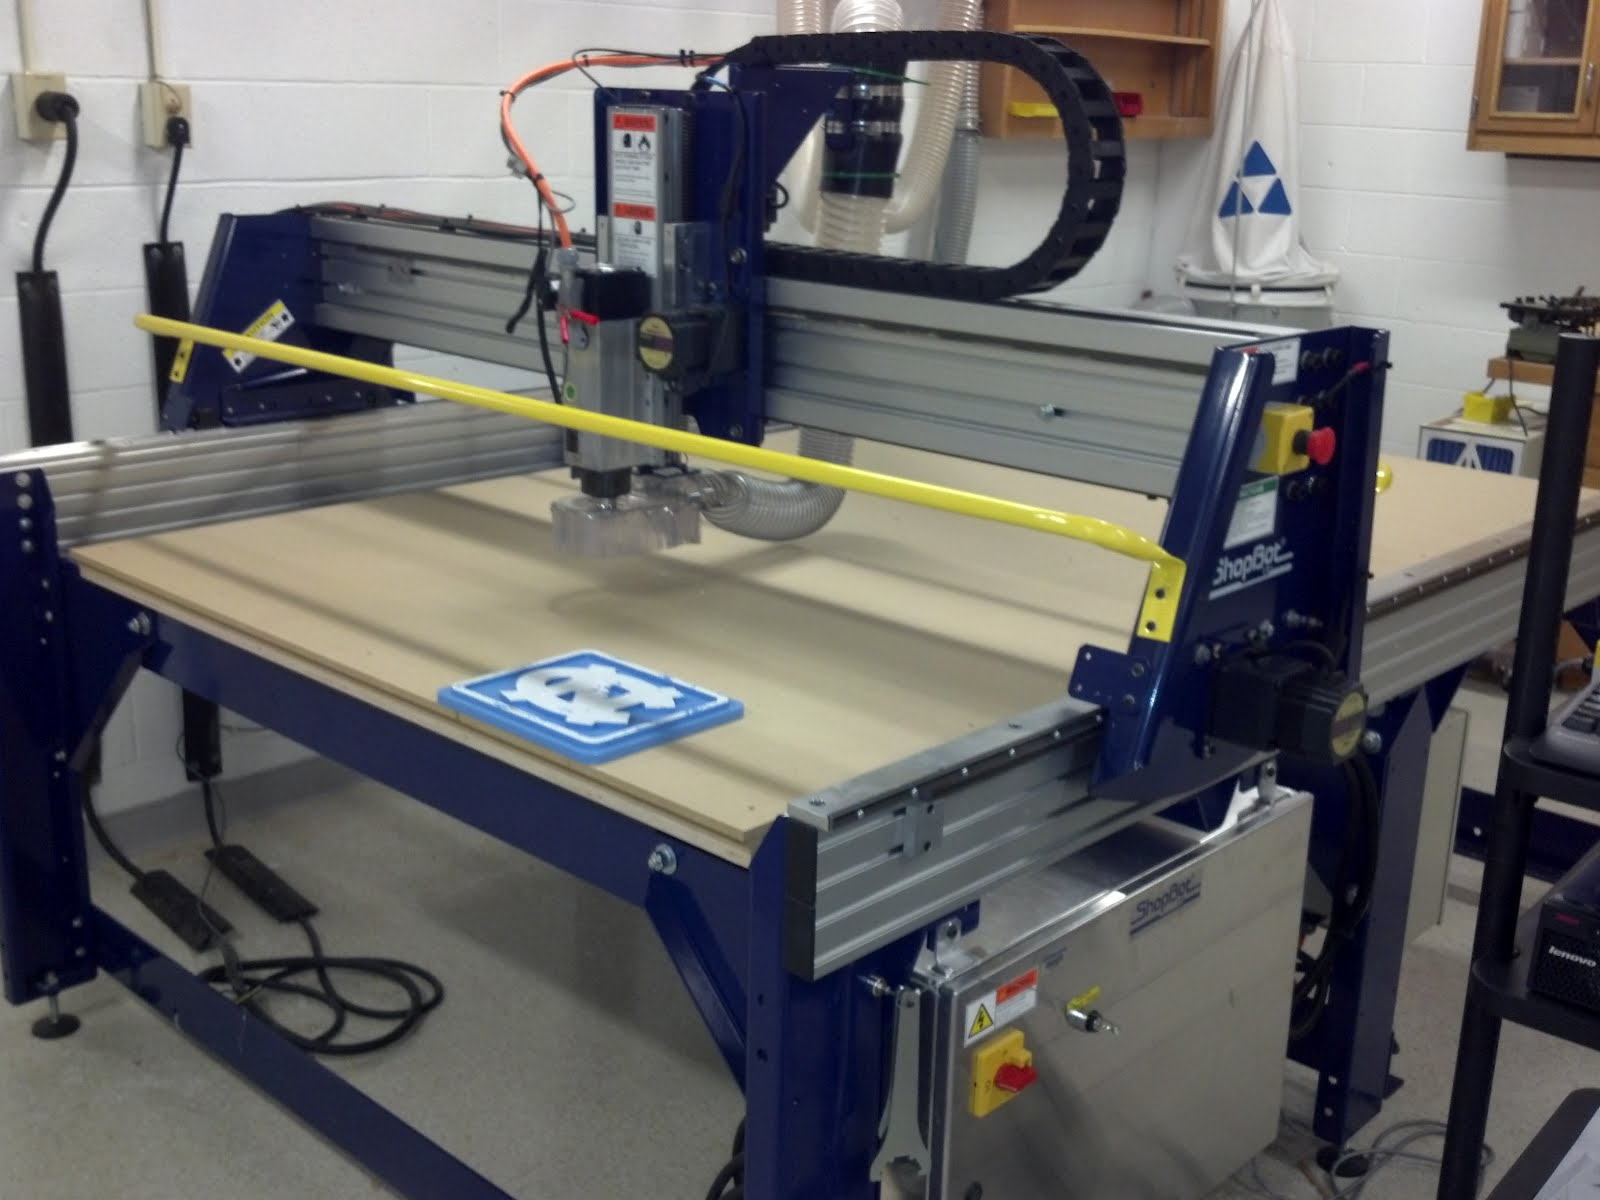
\includegraphics[width=0.7\linewidth]{img/ShopBot}
		\end{figure}
		The ShopBot needs to solve (almost) this every day
	\end{frame}
	\begin{frame}
		\frametitle{Approaches}
		\centering
		\footnotesize
		\begin{tabular}{|c|c|c|}
			\hline 
			\textbf{Algorithim} & \textbf{Complexity} & \textbf{Approximation} \\ 
			\hline\hline
			Brute-force & $O(V!)$ & 1 \\ 
			\hline 
			Held-Karp & $O(V^22^V)$ & 1 \\ 
			\hline 
			Greedy & $O(V\lambda)$, not all TSP's & 1.25 (for $D=2$) \\ 
			\hline 
			Christofides & $O(EV^{2.376})$ & 1.5 \\ 
			\hline 
			Ant colony (iterative)& $O(V\lambda)$ & Depends on G  \\ 
			\hline
			$m$-guillotine subdivision & $(O\left(n^{O(m)}\right)$ & $\left(1 + \frac{c}{m}\right)$ \\
			\hline
			PTAS & $O\left(V\left(\log V\right)^{\left(O\left(c\sqrt{D}\right)\right)}^{D-1}\right)$ & $1+\frac{1}{c}$\\
			\hline
		\end{tabular} 
	\normalsize
	Oh my, what do I choose for my algorithm, given my space/time constraints? (Probably the PTAS)
	\end{frame}
	\begin{frame}
		\frametitle{Some assumptions}
		\centering
		\begin{itemize}
			\item Approximate solutions are OK, but we want a lower bound
			\item The time an algorithm takes to complete (\texttt{\%\%timeit, \%\%time}) is a reasonable proxy to how complex an algorithm is
			\item Space complexity doesn't matter (otherwise Greedy starts to look like $O\left(V^2\lambda\log\lambda\right)$)
		\end{itemize}
	\end{frame}
	\begin{frame}
		\frametitle{Exact algorithm}
		\framesubtitle{Brute-force}
		\begin{block}{English explanation}
			Consider all tours of a graph $\rightarrow$ Sum their weights $\rightarrow$ take the argmin.
			How many tours are there of a graph? $O(V!)$
		\end{block}
		\begin{block}{Python}
			\tiny
			\begin{semiverbatim}
			 1 \ import itertools as it\newline
			 2 \ import networkx as nx\newline
			 3 \ import numpy as np\newline
			 4 \ \newline
			 5 \ def brute\_force(G):\newline
			 6 \ \quad tours = list(it.permutations(G.nodes())) \#O(V!)\newline
			 7 \ \quad costs = []\newline
			 8 \ \quad for tour in tours:\newline
			 9 \ \quad cost = 0\newline
			 10 \quad for n1, n2 in zip(tour, tour[1:]): \#O(V)\newline
			 11	\quad\quad	cost += G[n1][n2]['weight'] \newline
			 12 \quad	costs.append(cost) \newline
			 13 \quad return tours[np.argmin(costs)] 
			\end{semiverbatim}
		\end{block}
	\end{frame}
	\begin{frame}
		\frametitle{Exact algorithm}
		\framesubtitle{Brute-force}
		\centering
		We can reason about the approximation factor of 1 by looking how it improves iterativley with a slight tweak to the code, a stop after evaluating $n$ permutations out of $V!$\newline
		(figure to come)
	\end{frame}
	\begin{frame}
		\frametitle{Exact algorithm}
		\framesubtitle{Bellman-Held-Karp}
		\begin{block}{English explanation}
			TBD
		\end{block}
		\begin{block}{Mathematical formulation}
			\begin{align}
				\text{decision variable } x_E &== 1 \text{ if $x_E$ is on the optimal tour.}\nonumber\\
				\text{Minimize: } & \sum_{E} W_E \cdot x_E\\
				\text{Subject to: } \forall_V, &\sum_{E \subset adj(V)} x_E = 2\\
				\forall G' \subset G, &\sum_{E = V(G') \text{ to } V(G)} x_E \geq 2
			\end{align}
		\end{block}
	\end{frame}
	\begin{frame}
		\frametitle{Approximation algorithms}
		\framesubtitle{Greedy}
		\begin{block}{English explanation}
			Pick an arbitrary node $\rightarrow$ find the lowest-weight edge $\rightarrow$ travel down the edge if it leads to a node that the agent has not "visited" before. Terminate once all edges are visited.
		\end{block}
		\begin{block}{Algorithm}
			Start at a node $n \in V$, go down the edge $\forall m, min_W_{mn} adj(n)$ to pick a new node $m$, subject to $m\notin$ previous $n$.
		\end{block}
	\end{frame}
	\begin{frame}
		\frametitle{Approximation algorithm}
		\framesubtitle{Greedy}
		\centering
		Let's look at some data to see how the algorithm performs. This graph has the optimal tour cost of 2579. \begin{figure}
			\centering
			\includegraphics[width=0.7\linewidth]{"img/Simple greedy approach, small graph/scatter_vis"}
			\caption{$N$ is the starting node, the red, grey, and green lines denote worst, best and average case}
		\end{figure}
	\end{frame}
	\begin{frame}
		\frametitle{Approximation algorithm}
		\framesubtitle{Greedy}
		\centering
		It's distribution of costs is:
		\begin{figure}
			\centering
			\includegraphics[width=0.7\linewidth]{"img/Simple greedy approach, small graph/dist_across_cost"}
			\caption{Relative frequency vs cost (KDE interpolation)}
		\end{figure}
	\end{frame}
	\begin{frame}
		\frametitle{Approximation algorithm}
		\framesubtitle{Greedy}
		\centering
		And here's how the agent progresses through the greedy approach.
		\begin{figure}
			\centering
			\includegraphics[width=0.7\linewidth]{"img/Simple greedy approach, small graph/cost_progress_trace"}
			\caption{How the cost for the agent differs in time, each trace is a different starting node $N$.}
		\end{figure}
	\end{frame}
	\begin{frame}{TODO}
		run analysis of greedy agent average performance vs optimal tour to substantiate 1.25 approximation factor, rerun large graph analysis with new visualization code, build visualizations for $m$-guillotine subdivisions and provide a broken-down explination of the algorithim, write ant trail algorithim and run visualization code.
	\end{frame}
\end{document}